\documentclass{article}
\usepackage[utf8]{inputenc}
\usepackage{indentfirst}
\usepackage{multicol}
\usepackage{mathtools}
\usepackage{listings}
\usepackage{graphicx}
\graphicspath{ {./images/} }

\title{EE451 Final Project}
\author{Nathan Frank, Alex Baker, Grace Susanto}
\date{March 2021}

\begin{document}

\maketitle

\section{Introduction}
     \subsection{Problem}
            As the resolution of images increases with constant camera and display technology advances, there is a need for faster methods of doing basic kernel-based operations such as edge detection, sharpening, and blurring on these images as well as performing more advanced Computer Vision Algorithms such as a Hough Transform.  This problem is meaningful because as time goes on, image sizes and the need to rapidly process large sets of images will continue to increase.  In order to quickly compute these operations, efficiently employing multiple workers whether they be threads in a CPU or nodes in a network, will be necessary to keep the the processing time to an acceptable level.  However, the brute force approach of using as many threads as possible will often overshoot what is required for optimal speedup.  As higher thread count processors become more commonplace, the fastest calculation might not be with the largest amount of threads due to the accumulation of overhead on thread creation and exit.
            
            The problem being addressed by this project is the avoidance of overhead in parallelized image processing operations.  We will be parallelizing three algorithms, a basic edge detection kernel based algorithm, a Moravec corner detection algorithm, and finally a Hough transform algorithm.  We will be attempting to avoid the overhead of having too many threads by first defining each algorithm in a scalable way and then testing it for a large variety of threads in the range of 1 - 32 threads, the range of dedicated threads on common consumer hardware that is readily available in the year 2021.  After gathering the most optimal thread counts for an average image size using this testing method we will test if the values found are optimal on a smaller selection of images that were not part of the training data.  From the training data we will then try to create a model that takes the image size and complexity of desired operation into account when roughly approximating what amount of threads would result in the least amount of excess overhead.

    \subsection{Objective}
        Our primary objective was to train a model to predict the optimal thread count for three different image processing algorithms based on the size of the image measured in pixels. The three algorithms we chose are Moravec Corner Detection, Edge Detection, and a Hugh Transform. The algorithms will be discussed in depth later on.

\section{Workflow}
    \subsection{Languages and Libraries Used}
        We used C++11 as the primary language to carry out the project. We used pthreads (POSIX threads) for parallelization, and we used OpenCV (Computer Vision Library) to help with image processing.
        
    \subsection{Training}
        The first step to create our model was to divide our set of training images into groups based on their pixel counts. To do this, we used parallel k-means clustering of the images to group them appropriately. Once we had the images grouped together, the next step was to find the optimal thread count for each image and algorithm. To find the optimal thread count for a group of images, we ran our selected algorithms for every image using each thread count from 1-32. After determining the optimal (fastest) thread count for a given image and algorithm, we would update our model to reflect that (keep a running average of the optimal thread count for each cluster). After going through every image and every algorithm and finding the optimal thread counts, we stored the optimal thread counts for each algorithm and each cluster of images so that it could be used in the testing phase.
        
    \subsection{Testing}
        To test our model, we first loaded in a new set of testing images. We then used our model created in the training phase to predict the optimal thread count for each image. Next we ran each algorithm on each image using this predicted optimal thread count and recorded the execution time. To test if our predicted optimal thread count matches the actual optimal thread count, we then ran each algorithm on each image using all thread counts from 1-32 to calculate the actual optimal thread count and the worst-case thread count. 
        All of this data was then stored to be analyzed further outside of the code.
        
\section{Algorithms}
    \subsection{Data Partitioning}
        For all different algorithms of image processing where we needed to partition images for parallelization, we split the images vertically into pieces, or partition it using vertical decomposition. This allowed us to easily use any number of threads we wanted including odd numbers (as opposed to splitting the image into blocks). In order to prevent noise from occurring at the borders of our partitions, we pad each partition beyond the edge by one pixel. But instead of just padding the borders with 0, we extend by the pixel from the neighboring edge pixel of adjacent threads.
        \begin{center}
        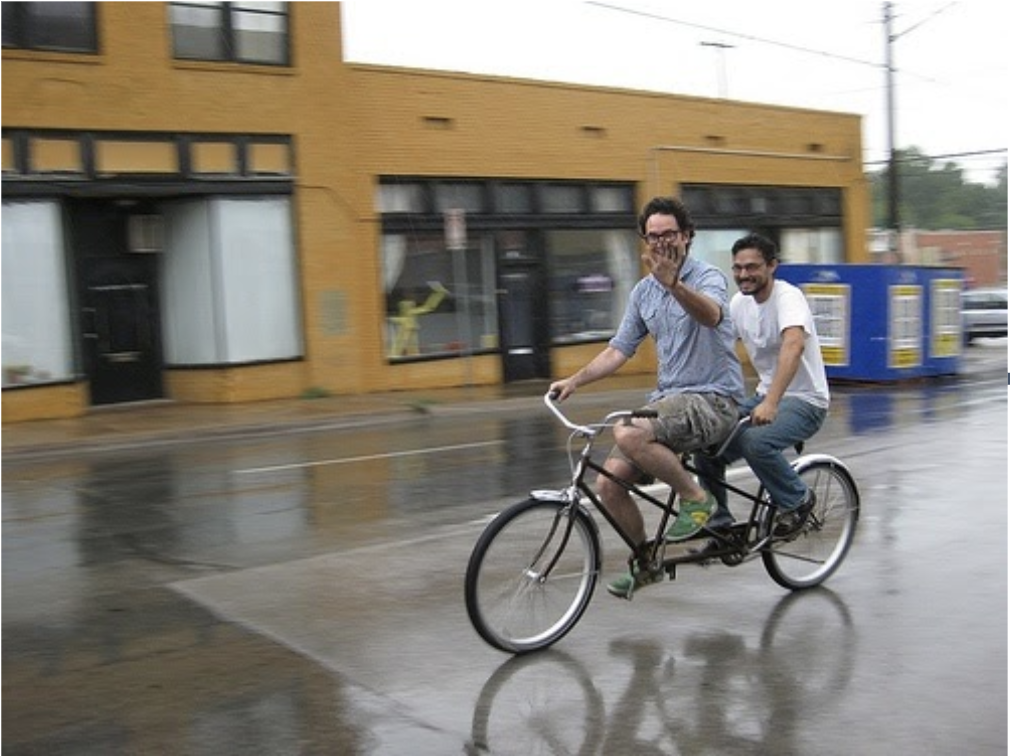
\includegraphics[width=0.45\textwidth]{source/images/vert-before.jpg}
        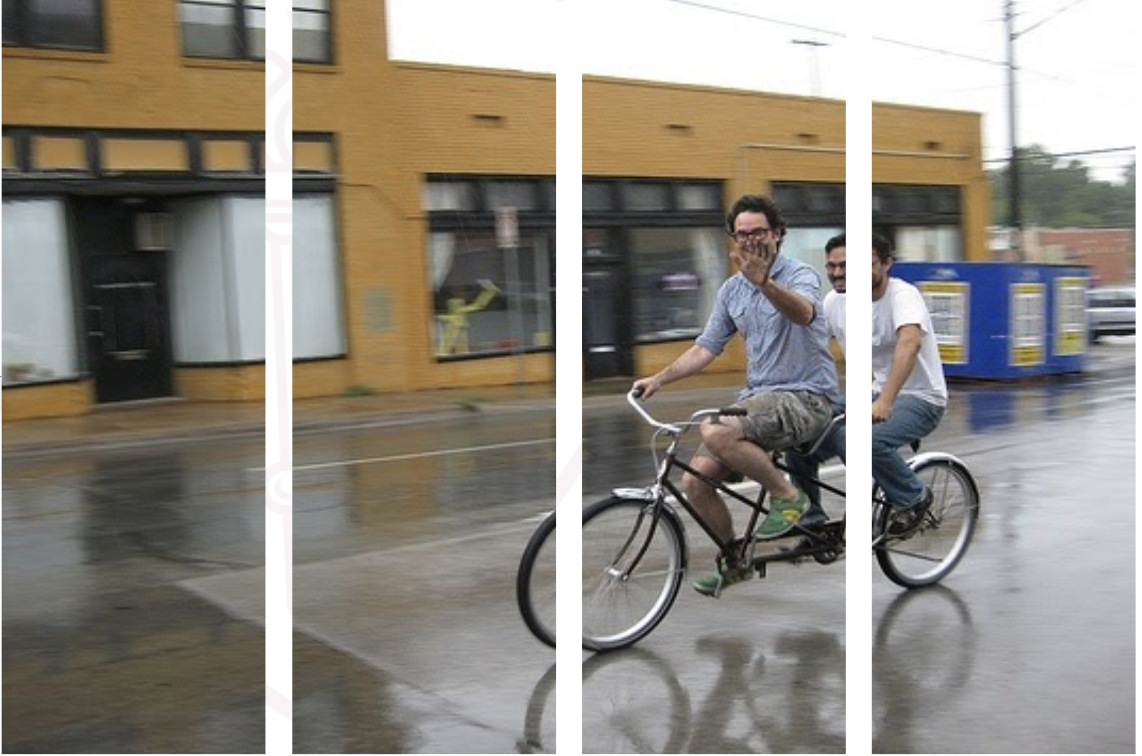
\includegraphics[width=0.45\textwidth]{source/images/vert-after.jpg}
        
        \caption{Vertical Decomposition Result}
        \end{center}
        
    \subsection{Sobel Edge Detection}
        Edges in images are places where there are strong intensity contrasts. To find these places we use a 'Sobel Filter' which finds the direction of the largest increase from light to dark and the rate of change in that direction. The results tell us how likely each pixel is to represent an edge. 
        First, we convert the image to grayscale. Then, using a 3x3 kernel we average each window to reduce the amount of noise present. We then apply the Sobel filter in both the x and y direction to get approximations of the change in intensity in both directions. Finally, we calculate the gradient magnitude at each pixel by combining the gradient approximations given by the Sobel Filter in the x and y directions. Once we have the gradient magnitude at each pixel, we apply a threshold function to only pick the peaks of the edges. Once we have determined which pixels are part of an edge, we assign those pixels to be white and everything else to be black to provide a visual representation of what the algorithm has done. In the example below, we have selected a sample image and the output from our edge detection algorithm. The three different colors represent the work done by different threads - in this case, three threads were used to perform the Sobel Edge Detection (colors are added for visualizing the partitions).
        \begin{center}
        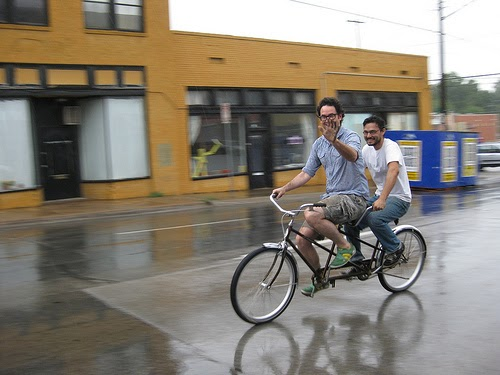
\includegraphics[width=0.45\textwidth]{source/images/edge_detection_before.jpg}
        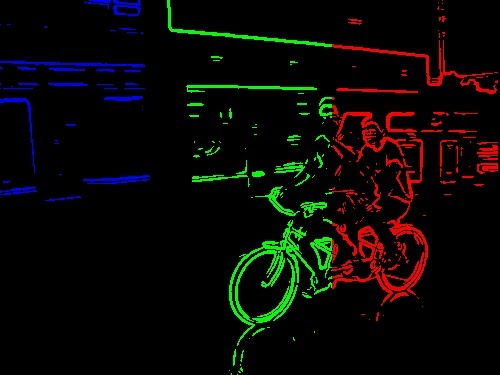
\includegraphics[width=0.45\textwidth]{source/images/edge_detection_complete.jpg}
        
        \caption{Sobel Edge Detection Result}
        \end{center}
        
        
    \subsection{Moravec Corner Detection}
        Corners in images are the intersections of two edges, a point for which there are two dominant and different edge directions in a local neighbourhood of the point. To find these places, we use Moravec Algorithm. In Moravec Algorithm,  a corner is defined to be a point with low self-similarity. The algorithm processes every pixel, determine its similarity with its surrounding region, then mark the possible corners. Out of these groups of possible corners, the algorithm will do a local maxima filter to get rid of closely grouped ones and get one point that will constitute as an edge. The similarity is measured by taking the sum of squared differences between the corresponding pixels of two patches. A lower number indicates more similarity. First, we convert the image to grayscale. Then, using a 3x3 kernel, compute the local intensity in each of the kernel. Then shift by 1 pixel in all directions in its surrounding 5x5 region, calculate the minimum squared difference for each shifts, and threshold that value. Finally, out of the possible corners, do a local maxima filter to get rid of closely grouped ones, so we get one point as the corner.
        \begin{center}
        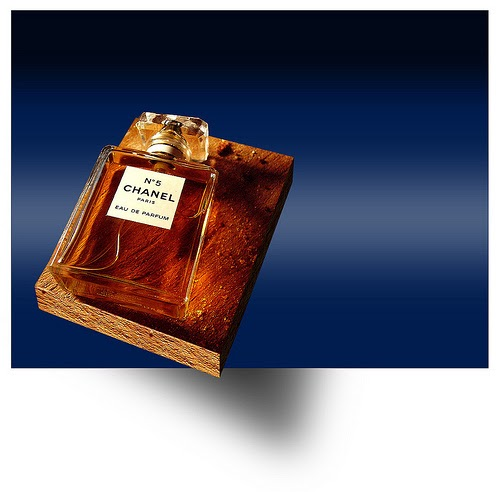
\includegraphics[width=0.45\textwidth]{source/images/moravec.jpg}
        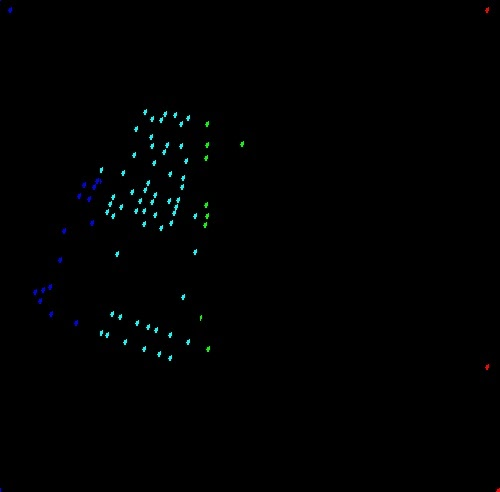
\includegraphics[width=0.45\textwidth]{source/images/moravec-after.jpg}
        
        \caption{Moravec Corner Detection Result}
        \end{center}
        
    \subsection{Hough Transform}
         Hough transform is a technique used to detect a feature or shape in an image. In this case, we want to detect a line in the image using Hough transform. A line can be represented as $y = mx+c$ or in parametric form, as $\rho = x * \cos\theta + y * \sin\theta$ where $\rho$ is the perpendicular distance from origin to the line, and $\theta$ is he angle between the $x$ axis and the line connecting the origin with that closest point.  Hough transform works by transforming an image into a 2D array called accumulator, or Hough space, that holds values of two parameters, $\rho$ as row and $\theta$ as column. A straight line $y = mx+c$ can be represented as a point $(m, b)$ in the accumulator. Given a single point in the plane, then the set of all straight lines going through that point corresponds to a sinusoidal curve in the ($\rho$, $\theta$) plane, which is unique to that point. A set of two or more points that form a straight line will produce sinusoids which cross at the ($\rho$, $\theta$) for that line. 
         
         Hough transform algorithm works by first running the edge detection algorithm, using Sobel Filter, on the image. Then, based on the edges points, if two different edges are in the same line, then they will intersect to a point in the Hough space, or in other words, those two points of the same line will fall into the same $\rho$ and $\theta$. Finally, Then, we perform groupings of edge points into object candidates by performing an explicit voting procedure over a set of parameterized image objects, that is for each edge pixel in the image x and y coordinate, we will increment by one (vote) its corresponding accumulator space $\rho$ and $\theta$ coordinate. After we have the local maxima of particular points in the accumulator space, we transform those points back to the x and y coordinate, and we will get the line detection.
         \begin{center}
        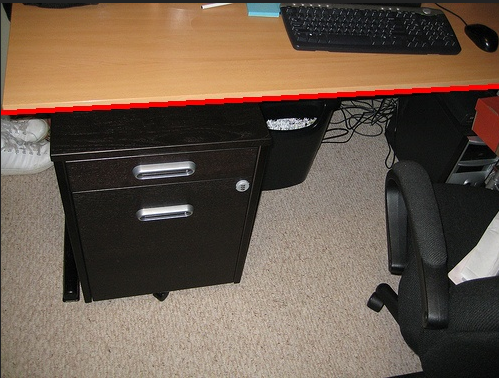
\includegraphics[width=0.45\textwidth]{source/images/unknown.png}
        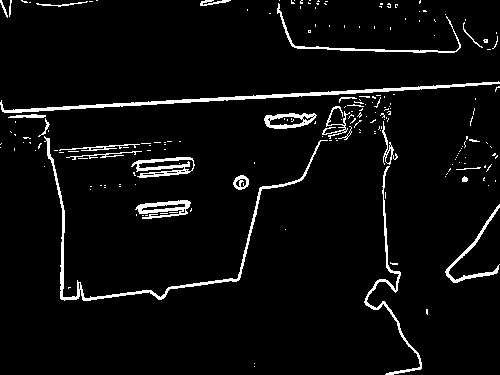
\includegraphics[width=0.45\textwidth]{source/images/testOutputEdge5.JPEG}
        
        \caption{Hough Transform Result}
        \end{center}
         
\section{Pseudocodes}
    \subsection{Data Partitioner and Thread Spawner Pseudo-Code}
        \begin{lstlisting}[basicstyle=\footnotesize]
        
for idx = {0, ..., thread_count - 1}:
    # Compute each thread' image region
    cols = image.columns / thread_count
    remainder = image.columns % thread_count
    for x = {idx*cols, ..., idx*cols + cols + remainder}:
        for y = {0, ..., image.rows}:
            # Construct the partitioned image for each thread plus padding
            input_image = the image in this range, with additional padding 
                in the border taken from the neighboring edge pixel of adjacent threads.
    # Spawn the thread to run specific algorithm using the constructed input image
    pthread_create (thread, algorithm, input_image)
 
 # Wait for each thread to finish and reconstruct resulting images by 
 # combining the resulting images from each thread
 for idx = {0, ..., thread_count - 1}:
    pthread_join (thread)
    reconstruct new image using the output partitioned image of each thread
    
        \end{lstlisting}
    
    \subsection{Sobel Edge Detection Pseudo-Code}
        \begin{lstlisting}[basicstyle=\footnotesize]

# Load the image in as an array of int[i][j][k]
rgb_image = load_image

# Convert image to grayscale array of int [i][j]
image = RgbToGrayscale(rgb_image)

# Using 3x3 kernels, average the window to reduce noise.
for x in cols:
    for y in rows: 
        Gb = average of pixel in 3x3 kernel of region surrounding image[x, y]
        image[x][y] = Gb
        
Gx_kernel = [{-1, 0, 1},{-2, 0, 2}, {-1, 0, 1}]
Gy_kernel = [{1, 2, 1}, {0, 0, 0}, {-1, -2, -1}]
for x in cols:
    for y in rows:
        # Apply the Sobel filter
        Gx = image[x][y] 3x3 kernel * Gx_kernel
        Gy = image[x][y] 3x3 kernel * Gy_kernel
        # Compute gradient magnitude, then assign edges pixel with 
        # white and non-edges pixel with black
        image[x][y] = (sqrt(Gx^2 + Gy^2)) > 150 ? 255 : 0
        
return image
        \end{lstlisting}
        
        \subsection{Moravec Corner Detection Pseudo-Code}
        \begin{lstlisting}[basicstyle=\footnotesize]
# Load the image in as an array of int[i][j][k]
rgb_image = load_image

# Convert image to grayscale array of int [i][j]
image = RgbToGrayscale(rgb_image)

for x in cols:
    for y in rows: 
        local_intensity = Sum of pixels centered in image[x][y] 3x3 kernel / 9
        shifted_intensity = Minimum of average pixel of 3x3 kernel 
            in the 5x5 kernel window centered at image[x][y]
        E = (shifted_intensity - local_intensity)^2
        if (E < 150) { image[x][y] = 0 }
        
        for every group of corners, pick the local maxima
        image[x][y] = image[x][y] is local maxima ? 255 : 0
        
return image

        \end{lstlisting}
        \subsection{Hough Transform Pseudo-Code}
        \begin{lstlisting}[basicstyle=\footnotesize]
        
# Load the image in as an array of int[i][j][k]
rgb_image = load_image

# Do Edge Detection resulting in black and white image with white as edges
image = SobelEdgeDetection(rgb_image)

for x in cols:
    for y in rows: 
        if (image[x][y] == 255) 
            for (theta = {0, ..., 180}) 
                # Do voting on accumulator space based on the edges 
                # from Sobel Filtered image
                int p = x * cos(theta) + y * sin(theta)
                accumulator_space[theta][p] += 1;

return accumulator_space
        \end{lstlisting}


\section{Results}
    \subsection{Sobel Edge Detection}
    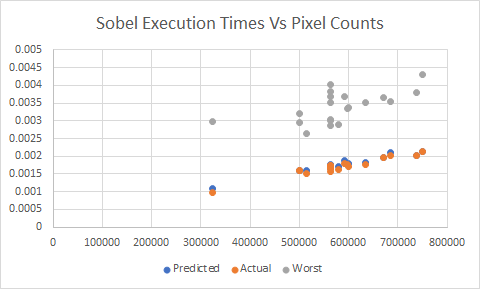
\includegraphics[width=\textwidth]{source/images/edge_detection.png}
    On the x-axis of the graph above, we have pixel counts, and on the y-axis we have the execution time in seconds. The blue dots represent the execution time using our predicted optimal thread counts, the orange dots represent the execution time using the actual optimal thread count (the lowest execution time we were able to achieve using 1-32 threads), and the grey dots represent the execution time using the worst-case thread count of 32. The first thing to notice in the results for Sobel Edge Detection is that our predicted optimal thread count always performed noticeably better than the worst case thread count. Our predicted optimal thread count consistently performed almost as well as the actual optimal thread count - the average difference between these two values across all test images was just 3.5275E-05s. On average, our predicted optimal thread count saved 0.00163884s compared to the worst case thread count, giving a speedup of 1.395x.  The predicted optimal thread count for the Sobel Edge Detection was 11 threads with each image in our test set
    
    \subsection{Moravec Corner Detection}
    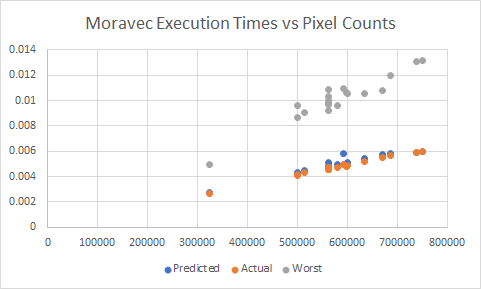
\includegraphics[width=\textwidth]{source/images/corner_detection.png}
    In the results for Moravec Corner Detection, our predicted optimal thread count always performed noticeably better than the worst case thread count. Our predicted optimal thread count consistently performed almost as well as the actual optimal thread count - the average difference between these two values across all test images was just 1.22385E-04s. On average, our predicted optimal thread count saved 0.00519479s compared to the worst case thread count, giving a speedup of 7.575x. The predicted optimal thread count for the Moravec Corner Detection was 9 threads with each image in our test set
    
    \subsection{Hough Transform}
    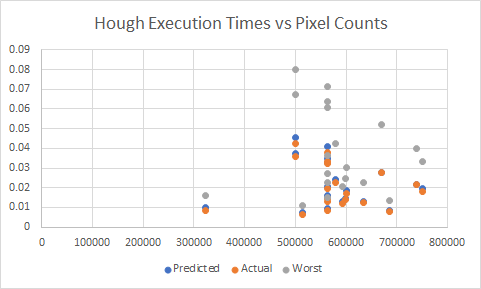
\includegraphics[width=\textwidth]{source/images/hugh_transform.png}
    In the results for Hough Transform, our predicted optimal thread count always performed noticeably better than the worst case thread count. Our predicted optimal thread count consistently performed almost as well as the actual optimal thread count - the average difference between these two values across all test images was just 0.00182846s. On average, our predicted optimal thread count saved 0.01607794s compared to the worst case thread count, giving a speedup of 2.12x. This is slightly worse speedup than the other algorithms because Hough transform requires a higher computational power to transform coordinate into accumulator space. The predicted optimal thread count for the Hough Transform was 4 threads with each image in our test set
    
    \subsection{Observation}
    We need to further research into the logarithmic regression to avoid entirely the training phase by knowing how fast our system is, how complex our algorithm is, and how much data we have. We also observe that we have a lot of noise when running our training phase due to Intel's Turbo boost technology that was sometimes inconsistent, so we decided to run the training phase three times and get the average of the result.

\begin{center}
\begin{table}
\begin{tabular}{|p{3cm}||p{3cm}|p{3cm}|p{3cm}|}
 \hline
 Algorithm Name & Average between Predicted and Actual & Average Time Saved over Worst Case & Average Speedup \\ 
 \hline
 \hline
 Sobel Edge Detection & 3.5275E-05s & 0.00163884s & 1.395x \\  
 \hline
 Moravec Corner Detection & 1.22385E-04s & 0.00519479s & 7.575x \\
 \hline
 Hough Transform & 0.00182846s & 0.01607794s & 2.12x \\
  \hline
\end{tabular}
\caption{\label{tab:table-name}Comparison between Performance using predicted thread count against actual optimal thread count case and worst case (32 threads).}
\end{table}
\end{center}


    \subsection{Overall Results and Discussion}
    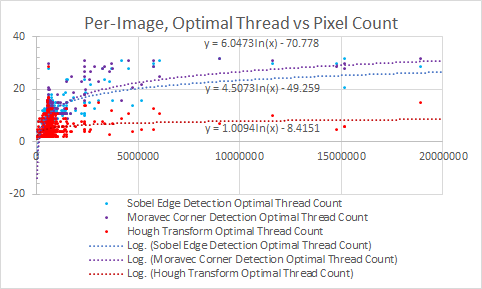
\includegraphics[width=\textwidth]{source/images/logarithmic_graph.png}
    This is the result of the training phase using 1500 images of different pixel count. Each data point represents the optimal thread count for each image for each algorithm. This is a Predicted Optimal Thread Count (y-axis) vs. Pixel Count graph (x-axis). We found that there is a logarithmic regression in the number of optimal thread count given the size of the input image.

\section{Challanges}
\begin{enumerate}
  \item Deciding how to group the image
  \begin{itemize}
     \item Deciding whether to group them by pixel count or horizontal or vertical decomposition or blocks
   \end{itemize}
  \item Learning OpenCV for managing the image data
  \item How to parallelize the data? Block vs. Column
  \begin{itemize}
     \item We decided to use column because it allows for more thread configurations, but we need to add padding to last thread
   \end{itemize}
   \item Splitting images into distinct parts and then recreating them without noise
   \begin{itemize}
     \item This is because we need to add padding around each of the split images for our 3x3 kernel to work, and we take the padding from each thread's neighboring thread images
   \end{itemize}
   \item Running on our local machines - inconsistent execution times
   \begin{itemize}
     \item We overcome this challenge by running each iteration multiples times to get an average execution time
   \end{itemize}
\end{enumerate}
        
\section{Further Exploration}
    \subsection{Grouping Images}
    In our project, we grouped images based on total pixel count. Further research would be needed to test if this technique is optimal or not. Another logical way to group images given that we partition the images vertically would be to use the width of the image measured in pixels rather than the total pixel count. This could potentially allow us to predict optimal thread counts more accurately since it aligns better with the method we used to partition the images.
    
    \subsection{Data Parallelism}
    In our project, we used data parallelism by partitioning images into vertical columns and having different threads operate on each column. Again, further research would be needed to test if there is a different method of partitioning that would give more accurate predictions for optimal thread counts. One other method to consider would be to partition the image into blocks instead of columns. This would help account for the fact that some images have different ratios of height to width, however it would also increase the complexity of partitioning the images, and it would make it impossible to partition images evenly with all thread counts from 1-32 (or it would require an uneven workload among the threads). One advantage of the approach we chose is that every image can be almost exactly (and easily) evenly partitioned for any number of threads.
    
    \subsection{Task Parallelism}
    Another path for future exploration would be to use task parallelism instead of or in addition to data parallelism. One example of how this could be implemented is in Sobel Edge Detection, we perform a Sobel Filter in both the x and y directions. In our project, since we only had one thread working on each partition of the image, the x and y direction filters were applied sequentially. Further research would be needed to test if additional speedup or more accurate predictions could be gained by instead assigning two threads to each partition such that one thread performs the filter in the x direction and the other thread performs the filter in the y direction. It's possible that this would result in slower execution times due to increased overhead and thread communication (the threads would have to synchronize and communicate in order to calculate the overall gradient magnitude for a given pixel), however it may be possible to optimize this approach such that the algorithm performs faster using this method of task parallelism.
    
    \subsection{Different Platforms for Parallelism}
    Another interesting path for future work would be to test our approach on different parallel coding platforms. We chose POSIX threads because they are available on most modern computers and do not require any additional hardware such as a GPU, but it would certainly be possible that using a different platform such as CUDA would change or improve the results of our predictions. This is especially relevant because in cases where large datasets of images are being processed, it will usually be on hardware better suited to image processing such as a GPU.
\end{document}
